\chapter{Daily Scrum Documentation}
\label{chap:dailyscrum}
\section{Cos'è il Daily Scrum?}
Lo scopo di questo documento è tenere traccia del lavoro giornaliero svolto da ogni membro del team. Nel nostro caso ogni team (Frontend e Backend) avrà il suo documento del Daily Scrum dedicato:
\begin{itemize}
    \item FE - Daily Scrum \href{https://studentiunimol-my.sharepoint.com/:x:/r/personal/a_daguanno1_studenti_unimol_it/_layouts/15/Doc.aspx?sourcedoc=\%7BC6890990-B5A6-4D9F-9306-993B687826C0\%7D&file=FE\%20-\%20Daily\%20Scrum.xlsx&action=default&mobileredirect=true}{[Drive Frontend]}
    \item BE - Daily Scrum \href{https://studentiunimol-my.sharepoint.com/:x:/r/personal/a_daguanno1_studenti_unimol_it/_layouts/15/Doc.aspx?sourcedoc=\%7BDC32CDAD-D25E-4F03-9490-1BA4A0895567\%7D&file=BE\%20-\%20Daily\%20Scrum.xlsx&action=default&mobileredirect=true}{[Drive Backend]}
\end{itemize}

Ogni Sprint ha la durata di 2 settimane di conseguenza il documento ha due tabelle da compilare nelle due settimane (week) ed i differenti fogli rappresentano i vari sprint che ci saranno durante il progetto.\\
Il primo sprint (\textbf{Sprint n.1}) va dal 30/03 al 12/04. E la prima settimana dal 30/03 al 05/04 \small{[fig:\ref{fig:week}]}

\begin{figure}[ht]
    \centering
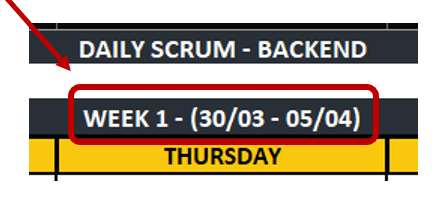
\includegraphics[width=0.7\textwidth]{Learning/09_ReadME_Documentazione/1_DailyScrumDoc/img_DSD/Immagine 2022-04-01 222626.png}
    \caption{suddivisione settimanale della tabella}
    \label{fig:week}
    \end{figure}
\FloatBarrier
\begin{figure}[ht]
    \centering
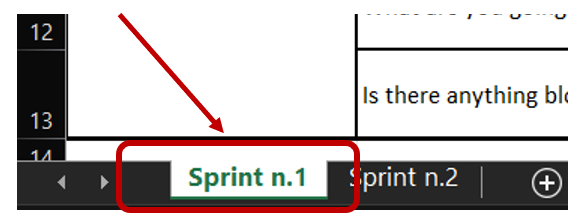
\includegraphics[width=0.7\textwidth]{Learning/09_ReadME_Documentazione/1_DailyScrumDoc/img_DSD/Immagine 2022-04-01 223141.png}
    \caption{fogli per la suddivisione degli Sprint}
    \label{fig:scrum}
    \end{figure}
\FloatBarrier

% ==============================================================================================================================
\newpage
\section{Come compilare il documento}
Ogni membro del team deve \underline{quotidianamente} rispondere alle 3 domande che compongono questo documento: 
\begin{enumerate}
    \item \textbf{What did you do yesterday?} - Descrivere ciò che è stato completato il giorno precedente.  
    \item \textbf{What are you going to do today?} - I progressi che si hanno in programma di fare.
    \item \textbf{Is there anything blocking you?} - Riportare i problemi che rallentano il workflow delle issue. 
\end{enumerate}

\subsection{Accedere al documento}
Ogni Team (FE e BE) ha una propria cartella dedicata sul Drive con tutti i file della documentazione relativi. I link sono presenti nel relativo canale \textbf{daily-scrum} del server Discord.\\
Il file si compila direttamente dall'editor online, in questo modo lavoriamo tutti sullo stesso file che sarà sempre aggiornato.\\
Chi vuole può creare una copia di backup che però non deve essere caricata nella cartella condivisa. 